\documentclass[Modultest/Modultest_main.tex]{subfiles}

\begin{document}
\section{GameController klassen på PlayerSideApp}\label{sec:GameController_modultest_bilag}
Denne modultest blev taget lavet sammen med den færdige RPI\_IF klasse på PlayerSideApp. Dette blev gjort, så det ikke var nødvendigt at lave stubs for denne klasse. Dette blev dog gjort for funktionerne controlAllLights og controlLight i CupLight\_IF klassen. Stubs bestod udelukkende af udskrivning til en UART, der blev tilføjet projektet, da det er en god måde, at teste om funktionerne bliver kaldt.CupSensor\_IF bruger GameController klassens funktioner updateCupStatus og updateHitStatus, og derfor skulle der også findes en metode, hvorpå de ville blive kaldt, som de ville i det samlede system. Her blev UART komponenten allerede tilføjet brugt endnu engang. UART komponenten blev tilføjet et interrupt på RX benet. Ved et tastetryk ville tasten trykket nu skabe et interrupt, hvorefter en handleByteReceived funktion ville kaldes, der læser tasten trykket og i et switch statement håndteres trykket. Her testes både om updateCupStatus og updateHitStatus fungerer. Inden dette blev gjort var det første, der blev testet, GameControllerens håndtering af en "state" ændring fra RPI'en. I figur \ref{fig:IDLE_STARTING} ses to beskeder sendt til PSoC'en, hvor de nødvendige informationer for at se om gamecontrolleren fungerer korrekt bliver udskrevet på skærmen. Man kan se at setState bliver kaldt, hvor den rigtige case eksekveres, da state IDLE og STARTING udskrives ved hjælp af UART. CupLight\_IF funktionen controlAllLights bliver også kaldt med turnedOffLight, da systemet kommer i state IDLE og i state STARTING anmodes om CupStatus fra CupSensor\_IF og controllingLights bliver kaldt samt controlLight i CupLight\_IF(kaldes 8 gange i den integrede del blev bliver den kun kaldt 6 gange, da for loopet i controllling lights blev ændret til 6, fordi der kun er 6 kopper).
\begin{figure}[H]
    \centering
    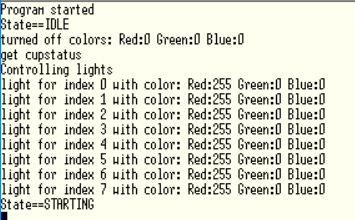
\includegraphics[width=0.5\textwidth]{Modultest/playerside_GameController/graphics/IDLE_STARTING.PNG}
    \caption{To "states" sendes til PSoC'en.}
    \label{fig:IDLE_STARTING}
\end{figure}

Når farvekode sendes til PSoC'en vil setMyColor eller setOpponentColor blive kaldt. Dette blev testet med funktionerne som stubs. Det var ikke nødvendigt at lave nye tests for disse, da stubs bare blev udvidet til at ændre MyColor og opponentColor variablerne i GameController og da dette er meget simpelt blev, der ikke gjort meget ud af disse test. I figur \ref{fig:farvekode_GameController} ses en ændring af farverne, men er bare samme test som blev lavet i RPI\_IF modultesten.
\begin{figure}[H]
    \centering
    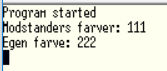
\includegraphics[width=0.5\textwidth]{Modultest/playerside_GameController/graphics/farvekode.PNG}
    \caption{Farven for MyColor og opponentColor ændres.}
    \label{fig:farvekode_GameController}
\end{figure}

\textbf{Test af updateCupStatus og updateHitStatus}
I denne test blev først updateCupStatus testet. Dette blev gjort ved at tasten 2 to på tastaturen blev trykket. Her er det kun updateCupStatus, der bliver kaldt i funktionen handleByteReceived funktionen i interrupt vektoren. Den bliver kaldt med CupStatus 0b11111100(updateHitStatus kaldes også men mded værdien 0, og der sker derfor ingen ændring), der betyder at 2 kopper er fjernet fra deres kopholder. Resultatet for denne ændring ses i figur \ref{fig:cupstatus_change}. Her ses det også at før denne update på CupStatus sker, så er der blevet skiftet til state PLAYING, hvor Cupstatus er 0b11111111. Dette ses ved at alle LED'er får den samme farve kombination. Efter CupStatus ændres har index 0 og 1 ændret farve kombination.
\begin{figure}[H]
    \centering
    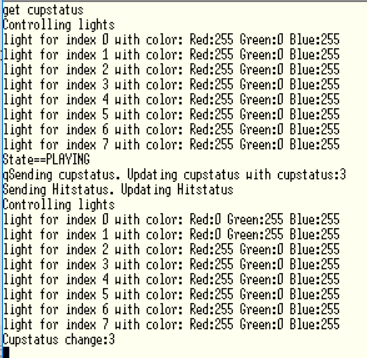
\includegraphics[width=0.5\textwidth]{Modultest/playerside_GameController/graphics/PLAYING_cupstatus_change.PNG}
    \caption{CupStatus ændres i state PLAYING.}
    \label{fig:cupstatus_change}
\end{figure}
Dette blev også testet i state STARTING, men det samme bliver udskrevet bortset fra, at det nu er missingCupColor og placedCupColor, der lyses med i stedet for MyColor og opponentColor. 
Efter dette var gjort med flere forskellige kombinationer af cupStatus skulle updateHitStatus testes. Dette blev gjort i state PLAYING, da der ellers ikke ville forekomme nogle ændringer i systemet. Vi skulle gerne se, at en timer begynder efter HitStatus er ændret. I figur \ref{fig:HitStatus_change} ses det at timeren begynder og der nu blinkes med myColor og opponentColor. For loopet i controllingLights blev sat ned til 4 for denne funktion, så der ikke blev udskrevet så meget til terminalen. Ved en ændring i state eller ved en ændring af HitStatus til 0 blev timeren stoppet.
\begin{figure}[H]
    \centering
    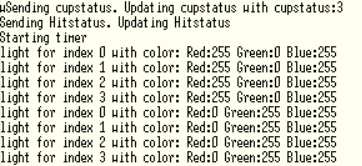
\includegraphics[width=0.5\textwidth]{Modultest/playerside_GameController/graphics/HIT_timer.PNG}
    \caption{HitStatus ændres, hvorved blink funktionen startes.}
    \label{fig:HitStatus_change}
\end{figure}
Dette var en god test, at have for timeren, som der i starten var problemer med, da den ville stoppe med at interrupte efter første gennemløb. Det viste sig at timerens status register har et flag, der bliver sat efter hvert interrupt. Dette flag fik vi nulstillet efter hvert interrupt og så virkede det, som det skulle.

\textbf{Løbende tests}
GameController klassen blev testet mange gange, da den var en central del af integrations testen af hele PlayerSideApp. Testene vist ovenfor er kun nogle af dem, der er blevet lavet, og små ændringer er fundet sted specielt i de stubs, der er blevet lavet. Det er altså ikke fuldstændig det samme kode, der var til modultest og som blev det færdige produkt, selvom modultesten var meget effektiv i at finde de største fejl, såsom timer fejlen beskrevet ovenover. 
\end{document}